\renewcommand*{\arraystretch}{1.1}

\noindent\begin{tabularx}{\queryCardWidth}{|>{\queryPropertyCell}c|X|}
	\hline
	query & Interactive / complex / 8 \\ \hline
%
	title & Recent replies \\ \hline
%
    pattern & \hfill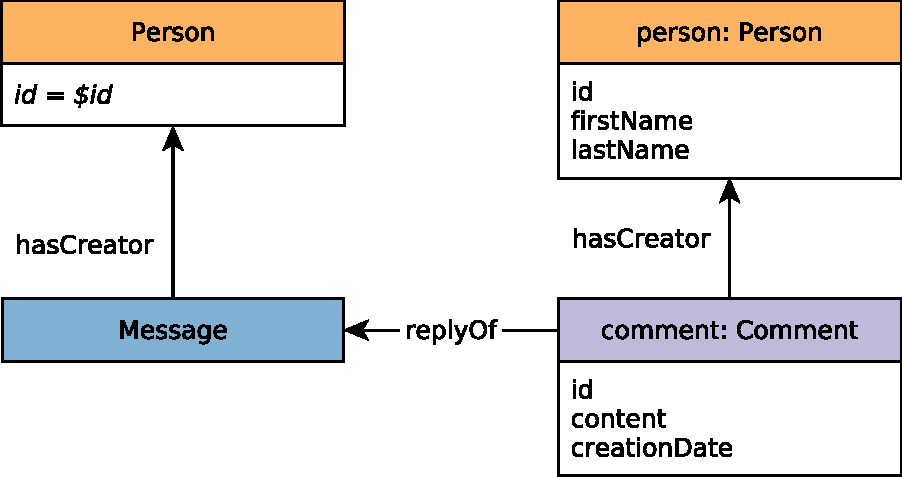
\includegraphics[scale=\patternscale,margin=0cm .2cm]{patterns/interactive-complex-read-08}\hfill\vadjust{} \\ \hline
%
	desc. & Given a start Person, find (most recent) Comments that are replies to
Messages of the start Person. Only consider immediate (1-hop) replies,
not the transitive (multi-hop) case. Return the reply Comments, and the
Person that created each reply Comment.
 \\ \hline
%
	
%
	params &
	\innerCardVSpace{\begin{tabularx}{\attributeCardWidth}{|>{\paramNumberCell}c|>{\varNameCell}M|>{\typeCell}m{\typeWidth}|Y|} \hline
	\cellcolor{parameter} \color{white} \footnotesize $\mathsf{1}$ &Person.id& ID &  \\ \hline
	\end{tabularx}}\innerCardVSpace \\ \hline
%
	
        result &
        \innerCardVSpace{\begin{tabularx}{\attributeCardWidth}{|>{\resultNumberCell}c|>{\varNameCell}M|>{\typeCell}m{\typeWidth}|>{\resultOriginCell}c|Y|} \hline
        $\mathsf{1}$ & Person.id & ID &R&
                 \\ \hline
        $\mathsf{2}$ & Person.firstName & String &R&
                 \\ \hline
        $\mathsf{3}$ & Person.lastName & String &R&
                 \\ \hline
        $\mathsf{4}$ & Comment.creationDate & DateTime &R&
                 \\ \hline
        $\mathsf{5}$ & Comment.id & ID &R&
                 \\ \hline
        $\mathsf{6}$ & Comment.content & String &R&
                 \\ \hline
        \end{tabularx}}\innerCardVSpace \\ \hline
	
%
	sort        &
        \innerCardVSpace{\begin{tabular}{|>{\sortNumberCell}c|>{\varNameCell}l|>{\directionCell}c|} \hline
        $\mathsf{1}$ & Comment.creationDate & $\desc$ \\ \hline
        $\mathsf{2}$ & Comment.id & $\asc$ \\ \hline
        \end{tabular}}\innerCardVSpace \\ \hline
	%
	limit & 20 \\ \hline
	%
	CPs &
	\multicolumn{1}{>{\raggedright}l|}{
	    \chokePoint{2.4}, 
	    \chokePoint{3.2}, 
	    \chokePoint{3.3}, 
	    \chokePoint{5.3}
	    } \\ \hline
	%
    relevance &
        \small This query looks for paths of length two, starting from a given Person, going through its created Messages and
finishing at their replies. In this query there is temporal locality between the replies being accessed. Thus the top k
order by this can interact with the selection, i.e. do not consider older posts than the 20th oldest seen so far.
 \\ \hline%
\end{tabularx}
\queryCardVSpace